\documentclass[border=1pt]{standalone}

\usepackage{tikz}
\usepackage{luatexja}
\usepackage{amsmath}

\usepackage{pgfplots}

\pgfplotsset{compat=1.18}

\begin{document}

    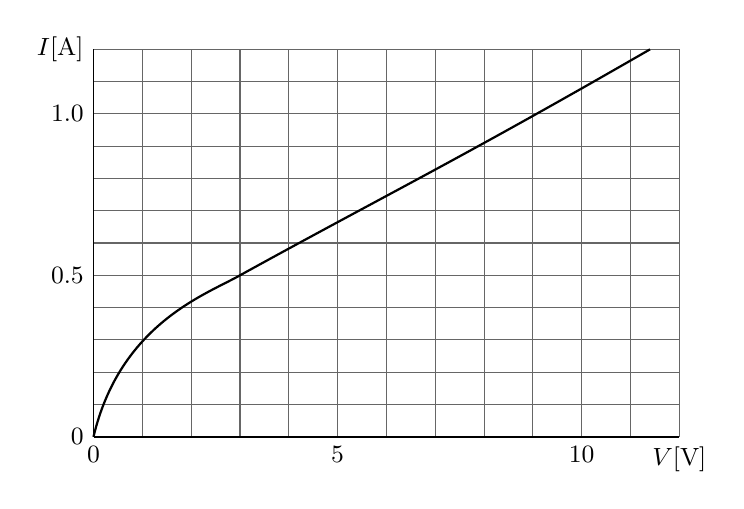
\begin{tikzpicture}[x=0.62cm, y=0.41cm]

        \pgfmathsetmacro{\X}{12}
        \pgfmathsetmacro{\Y}{12}

        % 1. 細かな方眼（グリッド）の描画
        \draw[step=1.0, black!60] (0,0) grid (\X,\Y);

        % 2. 軸と目盛り数値の描画
        \draw[semithick] (0,0) -- (\X,0) node[below, font=\small] {$V$[V]};
        \draw[semithick] (0,0) -- (0,\Y)
            node[left=, font=\small] {$I$[A]};

        % x軸目盛り
        \foreach \x in {0,5,10}
            \node[below, font=\small] at (\x, 0) {\x};

        % y軸目盛り (0.0, 0.1, ..., 1.1)
        \node[left, font=\small] at (0, 0){0};
        \foreach \y in {5,10}
            \node[left, font=\small] at (0, \y)
            {\pgfmathparse{\y/10}\pgfmathprintnumber[fixed, precision=1, zerofill]{\pgfmathresult}};

        % 3. 特性曲線の描画（全体を滑らかに結ぶ）
        % 各点での接線の傾きを調整し、曲線を再現
        \draw[thick] (0,0) 
            .. controls (0.55,3.5) and (2.3,4.4) .. (3,5)
            .. controls (6,7.5) and (7.5,8.6)  .. (11.4,12);
    \end{tikzpicture}
\end{document}
